\documentclass[a4paper]{article}

\usepackage[utf8]{inputenc}
\usepackage[T1]{fontenc}
\usepackage[francais]{babel}
\usepackage[top=1.5cm, left=2.5cm, bottom=1.5cm, right=2.5cm]{geometry}
\usepackage{amsmath}
\usepackage{amssymb}
\usepackage{textcomp}
\usepackage{graphicx}

\author{Théo Verhelst}
\title{Matière non-exhaustive pour l'examen du cours de Modélisation et Simulation}

\begin{document}
\maketitle
\section{Introduction}
Ce document reprend les questions/définitions listées par Mr. Bontempi comme étant des questions potentielles à son examen
oral, et y répond à partir des définitions du syllabus.
\paragraph{}
\emph{Note :} Toutes les définitions ne sont pas explicitées formellement, car Mr. Bontempi m'a assuré que seul
la compréhension des concepts est évaluée, pas la restitution pure des définitions.
\paragraph{}
\emph{Note :} Les variables et conventions de notations utilisées sont basées sur celles du syllabus.
\section{Définitions}
\begin{description}
	\item [Propriétés de la fonction de transition]:
		\begin{itemize}
			\item \emph{Consistance :} Si l'état du système au temps $t$ est $x$,
				la fonction de transition à l'instant $t$ doit donner $x$.
				\[\varphi(t,t,x,u(\cdot))=x\quad\forall t\in T, x\in X, u(\cdot)\in\Omega\]
			\item \emph{Irreversibilité :} $\varphi$ est définie pour tout \(t \ge t_0, t\in T\)
			\item \emph{Composition :} Si l'entrée $u(\cdot)$ fait évoluer l'état de $x_0$ à
				$\varphi(t_2,t_0,x_0,u(\cdot))$ durant $[t_0,t_2]$ en passant par $x(t_1)$,
				alors la même entrée fera passer l'état de $x(t_1)$ à $\varphi(t_2,t_0,x_0,u(\cdot))$
				durant $[t_1,t_2]$.
			\item \emph{Causalité :} Si deux fonction d'entrées sont identiques sur un intervalles,
				elles auront le même effet dans cette intervalle sur un système donné pour un état initial donné.
		\end{itemize}
	\item [Accessibilité]:\\
		Un état $x_2$ est \emph{accessible} à l'instant $t_2$ à partir d'un état $x_1$
		si $\exists\;t_1, u(\cdot)$ tels que \[\varphi(t_2,t_1,x_1,u(\cdot))=x_2\]
	\item [Observabilité]:\\
	\item [Notions de stabilité]:\\
		Un système est dit  \emph{stable} si une petite perturbation de son état initial
		n'induit pas une grande perturbation de son comportement au cours du temps.\\
		Plus formellement, un mouvement avec une condition initiale $\bar x$ est
		stable si pour tout voisinage $V_\epsilon$ de ce mouvement, on peut trouver
		une condition initale proche de $\bar x$ telle que le mouvement partant de
		cette condition initiale perturbée reste dans le voisinage $V_\epsilon$.
	\item [Critère de stabilité de Liapounov]:\\
		Soit un système à temps continu
		\[\dot x(t)=f(x(t),u(t))\]
		où le vecteur de fonctions $f(\cdot, \cdot)$ est continu ainsi que ses
		dérivées partielles.\\
		Soit $\bar x$ un état d'équilibre pour la fonction d'entrée constante $\bar u$.
		\begin{itemize}
			\item \emph{Critère de stabilité de Liapounov :} S'il existe une fonction
				$V(\cdot)$ continue (et que ses dérivées partielles sont également continues),
				qui soit définie positive en $\bar x$ et telle que la fonction
				\[\dot V(x)=\frac{dV(x)}{dt}
					=\sum_{i=1}^{n}\frac{\partial V}{\partial x_i}\dot x_i(t)
					=\Delta V(x)f(x,\bar u)\]
				où
				\[\Delta V(x)=\big[\frac{\partial V}{\partial x_1},\dots\frac{\partial V}{\partial x_n}\big]\]
				soit semi-définie négative en $\bar x$, alors $\bar x$ est un état d'équilibre stable.
			\item \emph{Critère de stabilité asymptotique de Liapounov :}
				Si le critère de stabilité de Liapounov est satisfait et que $\dot V(\cdot)$
				est définie positive (et non uniquement semi-définie positive) en $\bar x$,
				alors $\bar x$ est asymptotiquement stable.
			\item \emph{Critère d'instabilité de Liapounov :} Soit $V(\cdot)$
				une fonction continue (dont les dérivées partielles sont également continues)
				dans un voisinage de $\bar x$.
				Soit $V(\bar x)=0$ et positive dans un voisinage arbitrairement petit de $\bar x$.
				Si $V(\cdot)=\Delta V(x)f$ est définie positive en $\bar x$,
				alors l'état d'équilibre en $\bar x$ est instable.
		\end{itemize}
	\item [Propriétés des systèmes linéaires continus]:\\
		Définissons d'abord deux notions sur les mouvements:
		\begin{itemize}
			\item Le \emph{mouvement libre} est obtenu quand la fonction d'entrée est nulle ($u(\cdot)=0$).
			\item Le \emph{mouvement forcé} est obtenu quand la l'état initial est nul ($x(t_0)=0$).
		\end{itemize}
		Un système linéaire jouit des propriétés suivantes:
		\begin{itemize}
			\item Tout mouvement est la somme des mouvements libre et forcés correspondants.
			\item Si l'état initial $x_0$ est une combinaison linéaire $ax_{01} + bx_{02}$ de
				deux états initiaux, alors le mouvemement libre correspondant est la même
				combinaison linéaire des deux mouvemements libres correspondant à $x_{01}$ et $x_{02}$.
			\item Si la fonction d'entrée $u(\cdot)$ est une combinaison linéaire $au_1(\cdot) + bu_2(\cdot)$ de
				deux fonctions d'entrée, alors le mouvemement forcé correspondant est la même
				combinaison linéaire des deux mouvemements forcés correspondant à $u_1(\cdot)$ et $u_2(\cdot)$.
			\item La transformation de sortie $\eta$ est une fonction linéaire.
		\end{itemize}
	\item [Relation entre stabilité et le critère de Hurwitz]:\\
		Satisfaire le critère de Hurwitz est équivalent à prouver que le système
		est asymptotiquement stable.\\
		Le citère de Hurwitz se formulle comme suit:\\
		Soit le système linéaire invariant et autonome
		\[\dot x(t)=Ax(t)\]
		et soit
		\[\Delta_A(\lambda)=det(\lambda I - A) = \lambda^n+\sum_{i=1}^na_i\lambda^{n-i}\]
		son polynôme caractéristique. Posons
		\[H=\begin{bmatrix}
			a_1 & 1 & 0 & 0 & \dots \\
			a_3 & a_2 & a1 & 1 & \dots \\
			a_5 & a_4 & a_3 & a_2 & \dots \\
			a_7 & a_6 & a_5 & a_4 & \dots \\
			\vdots & \vdots & \vdots & \vdots & \\
		\end{bmatrix}
		\]
		où $a_{n+i} = 0 \forall i > 0$.\\
		Le critère de Hurwitz est satisfait si tous les mineurs principaux de $H$ sont positifs.
	\item [Principe de superposition des effets dans le cas d'un système
linéaire du second ordre]:\\
		\emph{\bf{Attention!}} Je ne suis pas sûre que ce théorème corresponde à cette définition! \\
		Soit le système
		\[\dot x=Ax\]
		et \(x^{(1)}(t)\in\mathbb{R}\) \(x^{(2)}(t)\in\mathbb{R}\)
		deux solutions linéairement indépendantes de ce système.
		\[\exists\,c_1,c_2\in\mathbb{C}\text{ t.q. }x(t)=c_1x^{(1)}(t)+c_2x^{(2)}(t)\]
		\(c_1\) et \(c_2\) sont déterminés en fonction des condition initiales.
	\item [Classifier la stabilité des systèmes de seconde ordre par
rapport à la matrice des coefficients]
		Soit le système
		\[\dot x=Ax\Leftrightarrow
		\begin{bmatrix}
			\dot x_1\\
			\dot x_2
		\end{bmatrix}
		=
		\begin{bmatrix}
			a_{11} & a_{12}\\
			a_{21} & a_{22}
		\end{bmatrix}
		\begin{bmatrix}
			x_1\\
			x_2
		\end{bmatrix}
		\]
		On a
		\[tr(A)=a_{11} + a_{22}\]
		\[det(A)=a_{11}a_{22} - a_{12}a_{21}\]
		On peut classer les systèmes en fonction de leur trace et de leur
		déterminant:\\
		\\
		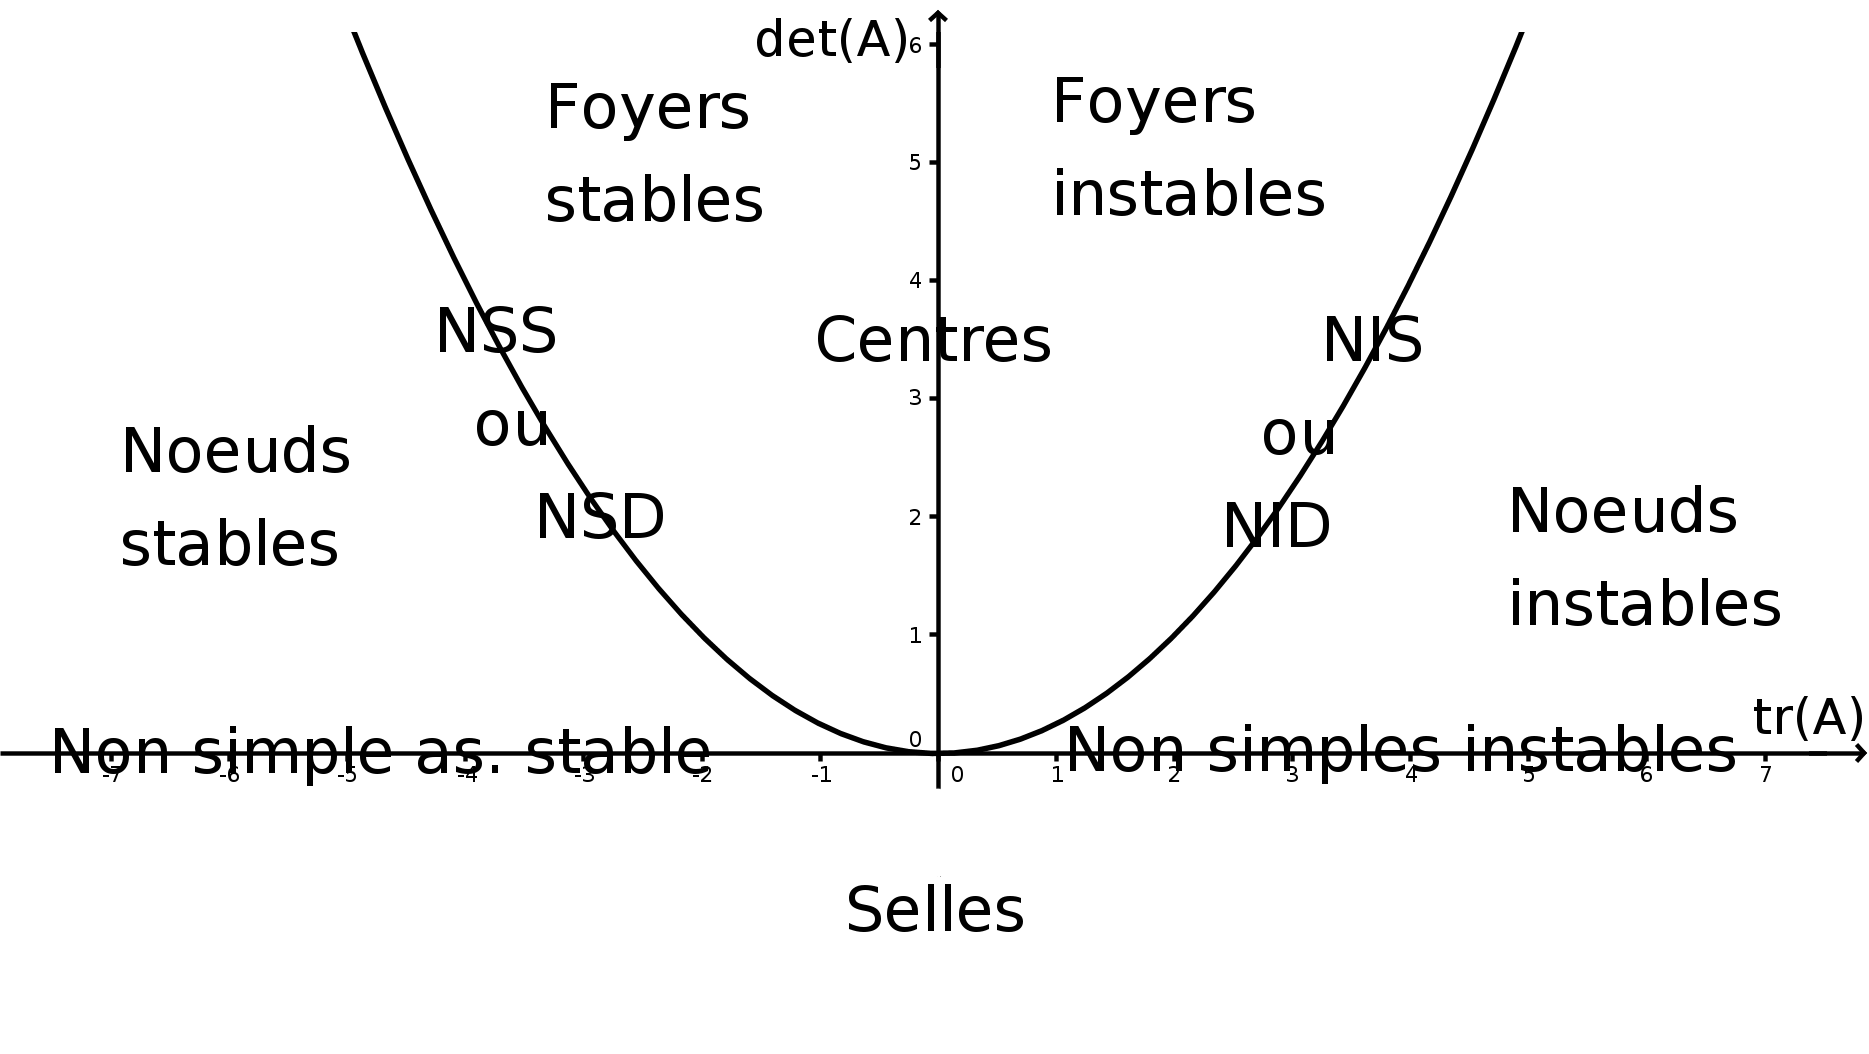
\includegraphics{graphic.png}\\
		\begin{description}
			\item[NSS]: noeuds stables singuliers
			\item[NSD]: noeuds stables dégénérés
			\item[NIS]: noeuds instables singuliers
			\item[NID]: noeuds instables dégénérés
		\end{description}
		La parabole des noeuds singuliers ou dégénérés est d'équation
		\[det(A)=\frac{(tr(A))^2}{4}\]
	\item [Relation entre linéarisation et stabilité]:\\
		Soit le système
		\[\dot x=f(x,u)\]
		avec un point d'équilibre \(\bar x\) et sa linéarisation en \(\bar x,\bar u\)
		\[
			\dot x=\left. \frac{\partial f}{\partial x}\right|_{\bar x,\bar u}x
			+\left. \frac{\partial f}{\partial u}\right|_{\bar x,\bar u}u
			=Ax+Bu
		\]
		\begin{itemize}
			\item Si le système linéarisé est asymptotiquement stable
				(c'est-à-dire toutes les valeurs propres de \(A\) sont négatives),
				alors l'état d'équilibre \(\bar x\) est asymptotiquement stable.
			\item Si la matrice \(A\) du système linéarisé a une ou plusieurs valeurs
			propres avec partie réelle positive, alors l'état d'équilibre \(\bar x\)
			du système est instable.
		\end{itemize}
	\item [Notion de diagramme de bifurcation]:\\
	\item [Cycle limite]:\\
	\item [Dimensionnalité d'un ensemble fractal]:\\
	\item [Système chatoique]:\\
	\item [Équation caractéristique et solutions d'un système linéaire à temps
discret]:\\
	\item [Étude graphique d'une équation linéaire affine à un pas]:\\
	\item [Relation entre linéarisation et stabilité]:\\
	\item [Diagramme de bifurcation de la fonction logistique]:\\
	\item [Composantes d'un algorithme Monte Carlo]:\\
	\item [Propriétés d'un générateur de nombre pseudo-aléatoires uniformes]:\\
	\item [Méthode de la transformation inverse]:\\
\end{description}
\end{document}
